\documentclass[a4paper, 10pt, final, onecolumn, openany, titlepage, twoside]{book}
\usepackage[nocap]{ctex} %% 中文宏包
\usepackage{fancyhdr} %% 负责控制页眉、页脚相关设置的宏包
\usepackage[text={150mm, 225mm}, left=30mm, vmarginratio=1:1]{geometry} %% 负责版面设计的宏包
\usepackage{graphicx} %% 和插图相关的宏包
\usepackage{amssymb, amsfonts, amsmath, amsthm, mathtools} %% 数学相关宏包
\usepackage{upgreek}
\usepackage{mathrsfs}
\usepackage{setspace} %% 调整行距的宏包
\usepackage{sectsty}
\usepackage[titletoc]{appendix}
\usepackage{listings} %% 代码展示宏包
\usepackage[usenames, dvipsnames]{xcolor} %% 颜色宏包
\usepackage{bigstrut} %% 该宏包提供 \bigstrut 命令,可以增大表格的行间距
\usepackage{array} %% 制表宏包
\usepackage{braket} %% Dirac bra and ket notation
\usepackage[colorlinks, linkcolor=blue, anchorcolor=red, citecolor=blue]{hyperref} %% 负责各种交叉引用的宏包
\usepackage[backend=biber, style=numeric-comp, sorting=none, maxbibnames=3, minbibnames=3]{biblatex} %% 文献处理宏包
\usepackage{ulem}
\usepackage[final]{pdfpages} %% 用于导入插入pdf文档的宏包
\usepackage[T1]{fontenc}
\usepackage[utf8]{inputenc} %% 输入字体编码宏包
\usepackage{lmodern} %% 英文字体宏包 (Latin Modern Roman, Latin Modern Dunhill, Latin Modern Sans Serif, Latin Modern Sans Typewriter)
\usepackage[english]{babel}




\pagestyle{fancy}  %% 页眉设置
\fancyhf{}
\fancyhead[OL]{\color{gray}\nouppercase\leftmark}
\fancyhead[ER]{\color{gray}\nouppercase\leftmark}
\fancyhead[EL, OR]{\thepage}
\fancypagestyle{plain}{\renewcommand{\headrulewidth}{0pt}\fancyhf{}}



\lstset{basicstyle=\footnotesize\ttfamily, columns=fullflexible, numbers=left, numbersep=5pt, numberstyle=\tiny, backgroundcolor=\color{white}, frame=single, breaklines=true, showtabs=false, showspaces=false, showstringspaces=false, keywordstyle=\color{teal}, commentstyle=\color{blue}, stringstyle=\color{red}, numberstyle=\color{gray}, tabsize=8, breakatwhitespace=false, postbreak=\mbox{\textcolor{violet}{$\hookrightarrow$}\space}}  %% 代码展示相关设置


\renewcommand{\ULthickness}{0.7pt} %% 设置封面中下划线的粗细程度


\chapternumberfont{\Huge}\chaptertitlefont{\huge}
\sectionfont{\Large}
\subsectionfont{\large}



\makeatletter  %% 自定义的引述环境
\newenvironment{PKUquote}[2][2em]
  {\setlength{\@tempdima}{#1}\def\chapquote@author{#2}\parshape 1 \@tempdima \dimexpr\textwidth-2\@tempdima\relax\itshape}
  {\par\normalfont\hfill--- \chapquote@author\hspace*{\@tempdima}\par\bigskip}
\makeatother




\addbibresource{Bibliography.bib} %% 加入参考文献库文件




\begin{document}



\def\ChineseTitle{用张量网络方法研究非平衡系统中涨落性质} % 中文标题
\def\EnglishTitleFirstLine{Tensor-Network Approaches to the Fluctuation Properties} % 英文标题第一行
\def\EnglishTitleSecondLine{in Nonequilibrium Systems} % 英文标题第二行
\def\author{顾加银} % 作者姓名
\def\StartTime{2021年6月} % 工作起始日期
\def\EndTime{2023年3月} % 工作期满时间
\def\SubmissionTime{2023年3月} % 报告提交时间
\def\FirstLevelSubjectName{北京大学物理学} % 流动站(一级学科)名称
\def\SecondLevelSubjectName{凝聚态物理} % 专业(耳机学科)名称
\def\institute{物理学院} % 院、系、中心




\begin{titlepage}
\begin{center}
\renewcommand{\ULdepth}{4pt}
\makebox[10mm]{} \\
\begin{minipage}{45mm}
\makebox[15mm]{\heiti\zihao{4}分\hfill 类\hfill 号}\uline{\makebox[40mm]{}}
\vspace{0.8cm} \\
\makebox[15mm]{\textbf{\zihao{4}U\hfill D\hfill C}}\uline{\makebox[40mm]{}}
\end{minipage}
\hspace{3.5cm}
\begin{minipage}{40mm}
\makebox[10mm]{\heiti\zihao{4} 密\hfill 级}\uline{\makebox[40mm]{}}
\vspace{0.8cm} \\
\makebox[10mm]{\heiti\zihao{4}编\hfill 号}\uline{\makebox[40mm]{}}
\end{minipage} \\
\vspace{3.2cm}
{\heiti\zihao{-2}\makebox[55mm]{北\hfill 京\hfill 大\hfill 学}} \\
\vspace{1.5cm}
{\heiti\zihao{-2}\makebox[85mm]{博\hfill 士\hfill 后\hfill 研\hfill 究\hfill 工\hfill 作\hfill 报\hfill 告}} \\
\renewcommand{\ULdepth}{10pt}
\vspace{2cm}
\uline{\heiti\zihao{4}\ChineseTitle} \\
\vspace{3cm}
{\heiti\zihao{4} 顾加银} \\
\vspace{1.5cm}
\renewcommand{\ULdepth}{5pt}
{\heiti\zihao{4}工作完成时间}\uline{\makebox[70mm]{\heiti\zihao{4}\StartTime  ---  \EndTime}} \\
\vspace{0.8cm}
{\heiti\zihao{4}报告提交时间}\uline{\makebox[70mm]{\heiti\zihao{4}\SubmissionTime}} \\
\vspace{0.8cm}
\makebox[20mm]{}\makebox[60mm]{\heiti\zihao{4} 北\hfill 京\hfill 大\hfill 学\hfill (北京)} \\
\vspace{0.8cm}
\makebox[30mm]{}\makebox[60mm]{\heiti\zihao{4} \SubmissionTime}
\end{center}
\end{titlepage}
\clearpage{\pagestyle{empty}\cleardoublepage}











\begin{titlepage}
\begin{center}
\makebox[10mm]{} \\
\vspace{0.8cm}
{\heiti\zihao{3}\ChineseTitle} \\
\vspace{2.3cm}
\textbf{\zihao{4}\EnglishTitleFirstLine} \\
\vspace{0.2cm}
\textbf{\zihao{4}\EnglishTitleSecondLine} \\
\vspace{1.7cm}
\begin{minipage}{60mm}
\makebox[60mm]{\heiti\zihao{4}博\hfill 士\hfill 后\hfill 姓\hfill 名:} \\
\vspace{0.5cm} \\
\makebox[60mm]{\heiti\zihao{4}流动站(一级学科)名称:} \\
\vspace{0.5cm} \\
\makebox[60mm]{\heiti\zihao{4}专\hfill 业(二级学科)名称:}
\end{minipage}
\hspace{-0.3cm}
\begin{minipage}{40mm}
{\heiti\zihao{4}\author} \\
\vspace{0.5cm} \\
{\heiti\zihao{4}\FirstLevelSubjectName} \\
\vspace{0.5cm} \\
{\heiti\zihao{4}\SecondLevelSubjectName}
\end{minipage} \\
\vspace{3cm}
{\heiti\zihao{4}研究工作起始时间:\StartTime} \\
\vspace{1cm}
{\heiti\zihao{4}研究工作期满时间:\EndTime} \\
\vspace{2.5cm}
\makebox[10mm]{}{\heiti\zihao{4}北京大学\institute(北京)} \\
\vspace{1.5cm}
\makebox[10mm]{}{\heiti\zihao{4}\SubmissionTime}
\end{center}
\end{titlepage}
\clearpage{\pagestyle{empty}\cleardoublepage}

 %% 封面
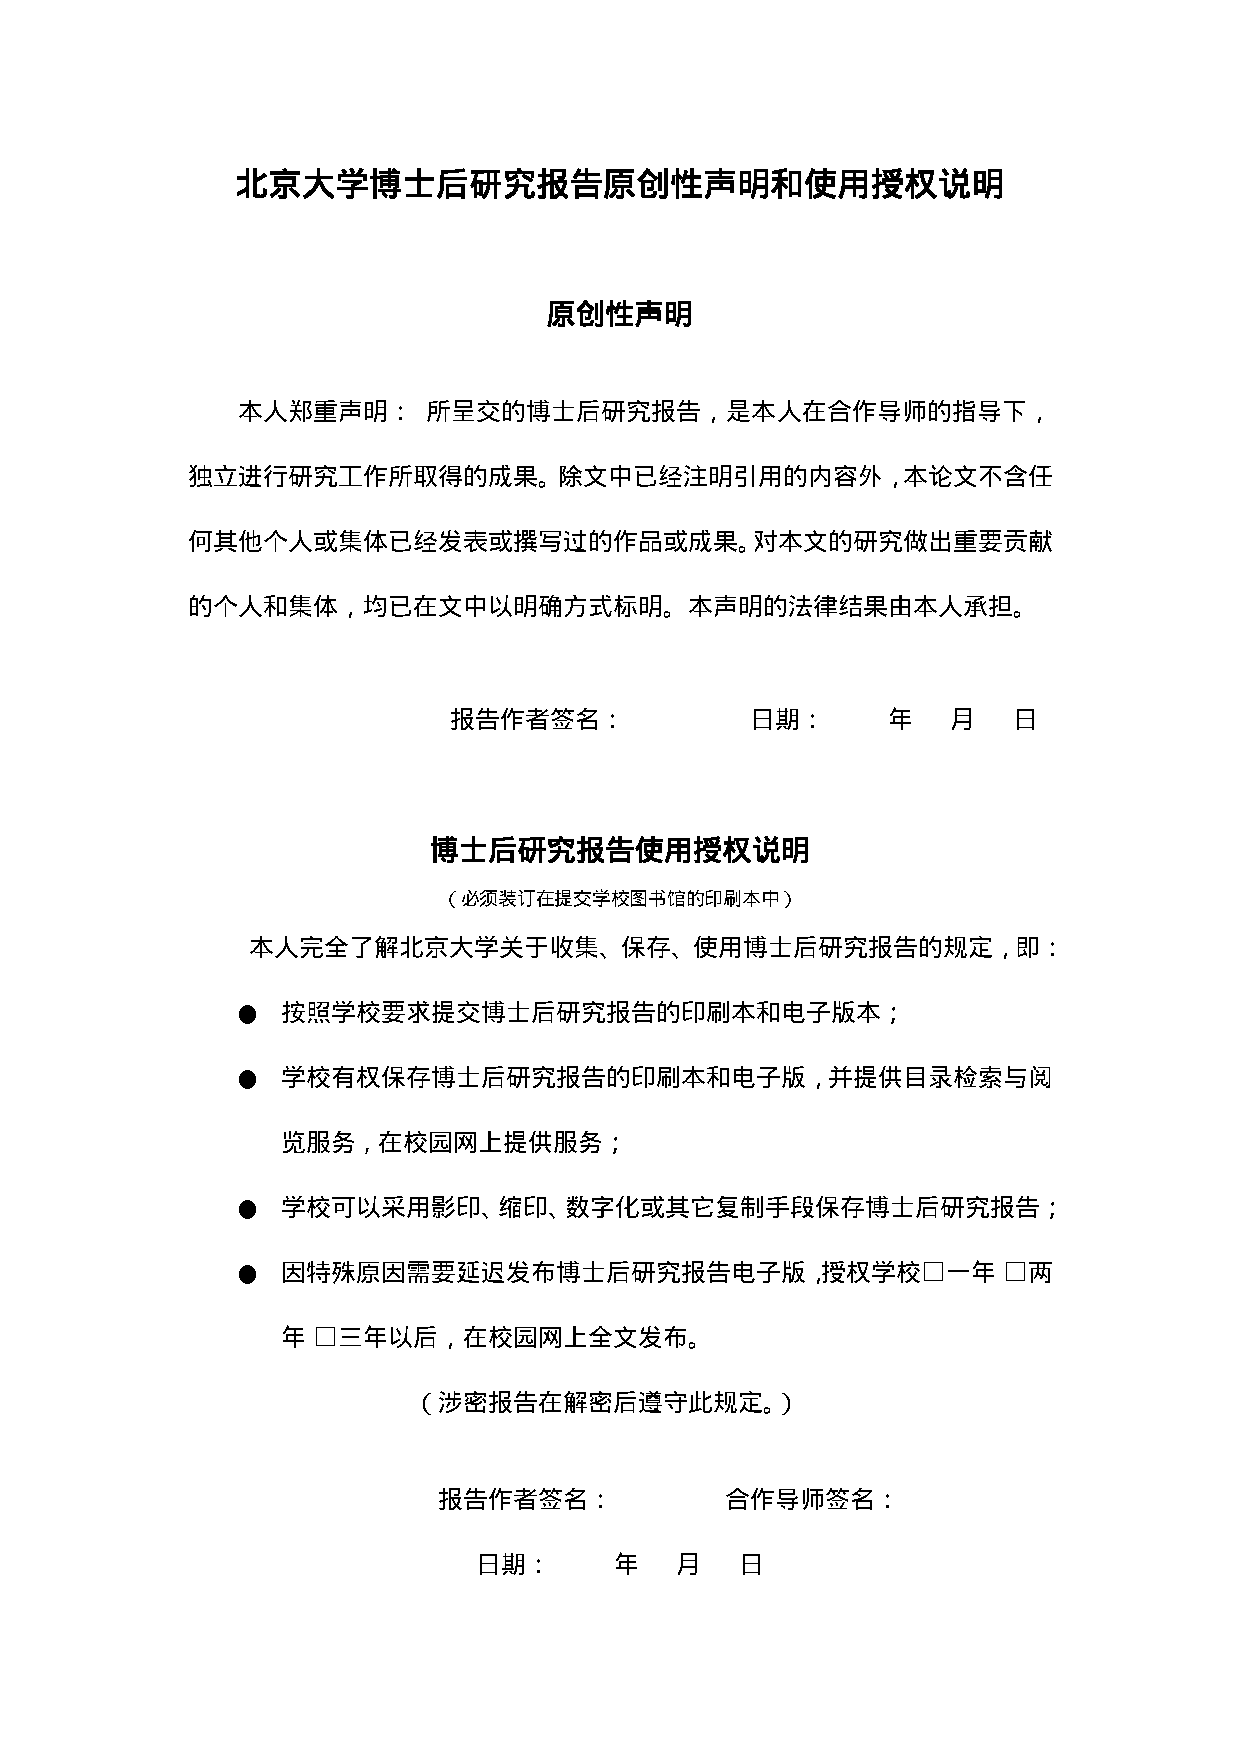
\includepdf{Declaration.pdf} %% 声明
\clearpage{\pagestyle{empty}\cleardoublepage}



\frontmatter


\chapter{Acknowledgements}

\begin{spacing}{1.5} %% set the seperation between lines
\par {\large First of all, I am grateful to Prof. H. T. Quan for his invitation that I got such an valuable opportunity to carry out my postdoctoral research in his group at Peking University. I am indebted to Dr. Jin Chen for his continuous support as a consultant about tensor networks, and Prof. Pierre Gaspard for his discussions and encouragement in the research. I would also like to thank my colleagues, Fan Zhang, Jinfu Chen, Yu-Xin Wu, Jihui Pei and many others. The pleasant interaction with them greatly enriched my daily life during the last two years. Finally but particularly, the financial support from Boya Postdoctoral Fellowship of Peking University and National Science Foundation of China under the Grants No. 12147162 is acknowledged.}
\end{spacing}
 %% 致谢
\chapter{\centering\heiti 内容摘要}


\begin{spacing}{1.5} %% set the seperation between lines
\par 在这份研究报告中我们展示张量网络是如何用来在数值上研究非平衡系统中的涨落性质。特别地,我们聚焦于这样的系统,他们的自由度随着系统尺寸呈现指数增长关系,而其中相关量的涨落可以用一些统称为涨落定理的漂亮关系式来量化。张量网络方法被用来计算涨落的特征函数,从这些函数中可以提取出更加细致的信息。 

\par 我们首先对于涨落定理给出一个简要的介绍。具体来说,我们在经典统计力学的框架中给出Jarzynski恒等式的推导,也基于马尔可夫随机动力学给出Gallavotti-Cohen涨落定理的推导。这两个关系式代表了非平衡物理在过去三十年的主要成就。

\par 然后,我们介绍一种张量网络方法,可以用来计算初始处于热平衡态的量子格点系统的功分布。在这个方法中,动力学演化用Time Evolving Block Decimation (TEBD)方法模拟,初始的热平衡态可以通过直接TEBD方法制备,也可以通过Minimally Entangled Typical Thermal States (METTS)方法制备,后者产生一系列典型的态来代表吉布斯正则系综。作为一个示例,我们将此方法应用于处于横场和纵场中的伊辛链。在给定驱动下,可以计算出功分布的矩生成函数,从中验证了量子Jarzynski恒等式和一个包含任意可观察量泛函的广义的量子功关系式。

\par 最后,我们将张量网络应用于对非平衡扩散系统中的随机粒子输运做计数统计。这个系统由一个一维的输运通道构成,两端分别接触粒子库。两种张量网络方法被用来实现这样一个应用,它们分别是Density Matrix Renormalization Group (DMRG, 密度矩阵重整化群)和TEBD。输运流的累计量生成函数被数值计算出来,并且和它们的解析解进行对比。我们发现了两者完美吻合,这充分说明了这些方法的有效性。此外,关于输运流的涨落定理也通过验证是成立的。
\end{spacing}
\vspace{5mm}
\noindent {关键词:非平衡物理,涨落定理,功分布,计数统计,张量网络方法}







\chapter{Abstract}

\begin{spacing}{1.5} %% set the seperation between lines
\par In this report we exhibit how tensor networks can be used to numerically investigate the fluctuation properties in nonequilibrium systems. In particular, we focus on the systems whose degrees of freedom grow exponentially with the system size, and in which the fluctuations of relevant quantities are quantified by some remarkable relations, collectively known as fluctuation theorem. Tensor-network approaches are applied to calculate the characteristic functions of fluctuations that more detailed information can be extracted from.

\par We start by giving a brief introduction to the fluctuation theorem. Specifically, we present the derivations of the Jarzynski equality in the framework of classical statistical mechanics, and of the Gallavotti-Cohen fluctuation theorem for the Markovian stochastic dynamics. These two relations represent the major advance in nonequilibrium physics in the last three decades.

\par Then, we introduce a tensor-network approach to calculate the statistics of work done on 1D quantum lattice systems initially prepared in thermal equilibrium states. In this approach, the dynamics is simulated with Time Evolving Block Decimation (TEBD), and the initial thermal equilibrium state is prepared either directly with TEBD or with Minimally Entangled Typical Thermal States (METTS), which generates a set of typical states representing the Gibbs canonical ensemble. As an illustrative example, we apply this approach to the Ising chain in mixed transverse and longitudinal fields. Under a prescribed protocol, the moment generating function for work distribution can be calculated, from which the quantum Jarzynski equality and the generalized quantum work relation involving a functional of an arbitrary observable are tested.

\par Finally, we apply tensor networks to counting statistics for the stochastic particle transport in an out-of-equilibrium diffusive system. This system is composed of a one-dimensional channel in contact with two particle reservoirs at the ends. Two tensor-network algorithms, namely, Density Matrix Renormalization Group (DMRG) and TEBD, are respectively implemented. The cumulant generating function for the current is numerically calculated and then compared with its analytical solution. Excellent agreement is found, manifesting the validity of these approaches in such an application. Moreover, the fluctuation theorem for the current is shown to hold.
\end{spacing}
\vspace{5mm}
\noindent {Keywords: Nonequilibrium Physics, Fluctuation Theorem, Work Statistics, Counting Statistics, Tensor-Network Approaches}
 %% 摘要
\begin{spacing}{1.1}
\tableofcontents %% 目录
\end{spacing}
\clearpage{\pagestyle{empty}\cleardoublepage}




\mainmatter

\def\path{Introduction}\chapter{Conclusion and Perspectives}


\par The present report has been devoted to study of the nonequilibrium systems with tensor-network approaches, with the focus on the fluctuation properties of relevant quantities. The characteristic functions quantifying the fluctuations are numerically calculated.















 %% 导论
\def\path{Fluctuation_theorem}\chapter{Conclusion and Perspectives}


\par The present report has been devoted to study of the nonequilibrium systems with tensor-network approaches, with the focus on the fluctuation properties of relevant quantities. The characteristic functions quantifying the fluctuations are numerically calculated.
















\def\path{Conclusion_and_perspectives}\chapter{Conclusion and Perspectives}


\par The present report has been devoted to study of the nonequilibrium systems with tensor-network approaches, with the focus on the fluctuation properties of relevant quantities. The characteristic functions quantifying the fluctuations are numerically calculated.















 %% 总结与展望



\begin{appendices}
\def\path{Appendices}


\chapter{Numerical Details and Code Implementations}\label{chap:code}


\begin{PKUquote}{Donald E. Knuth}
Computer programming is an art, because it applies accumulated knowledge to the world, because it requires skill and ingenuity, and especially because it produces objects of beauty. A programmer who subconsciously views himself as an artist will enjoy what he does and will do it better.
\end{PKUquote}





\noindent Computer programming plays an increasing important role in scientific research. It has de-facto become a pillar in scientific research, to be complementary with theory and experiment. A scientist might first build a model to describe a physical system according to the underlying physical laws, then use a computer to calculate the results and visualize them. This is now a widely adopted paradigm in scientific community. This appendix is devoted to the numerical details and code implementations about the DMRG approach to counting statistics. The required software and code written in C++ are presented in detail. Some explanatory remarks are also given.






\section*{Required Software}


The following listed software are those minimal requirements for the code presented in next section to be compiled and executed correctly.
\begin{itemize}
\item \href{https://releases.ubuntu.com/22.04/}{Ubuntu 22.04} -- one of the most popular distribution of Linux operating system. Other version might also be OK, but it is highly recommended to use the most recent one.
\item \href{https://gcc.gnu.org/}{g++} -- an open-source C++ compiler included in GCC (GNU Compiler Collection). It can be installed on Ubuntu with the command \texttt{sudo apt install g++}.
\item \href{https://www.gnu.org/software/make/}{GNU Make} -- a utility that facilitates compiling a program from source code. It reads from a file named \texttt{Makefile} which includes a set of instructions to be executed. It can be installed on Ubuntu with the command \texttt{sudo apt install make}. Readers are referred to Ref.~\cite{GrahamCumming_2015} for detailed account.
\item \href{https://www.gnu.org/software/gsl/}{GSL} (GNU Scientific Library) -- an open-source library for C/C++ programmers. It is licensed under the GNU General Public License (GPL). It can be installed on Ubuntu with the command \texttt{sudo apt install gsl-bin libgsl27 libgsl-dbg libgsl-dev}. The reference manual for this library is Ref.~\cite{GSL_manual_2021}.
\item \href{https://itensor.org/}{ITensor} (Intelligent Tensor) -- an open-source library for performing tensor computation. It provides both C++ and Julia version, whereas the former is used here. The installation instructions comes with the downloaded source code from \href{https://github.com/ITensor/ITensor}{here}. Readers are referred to Ref.~\cite{Fishman_SciPostPhysCodeb_2022} for more details.
\end{itemize}





\section*{C++ Code for DMRG Approach to Counting Statistics}


\par In the following, we show the code, which are written in separate text files:
\begin{itemize}
\item \texttt{Class\_model.h}.
\end{itemize}




\begin{spacing}{0.89} %% set the seperation between lines

\begin{lstlisting}[language=C++, caption={\texttt{Class\_model.h}.}]
#include <iostream>
#include <fstream>
#include <iomanip>
#include <cmath>
#include <vector>
#include <itensor/all.h>

class Cmodel
{
	public:
		static itensor::Real m_D;
		static itensor::Real m_Delta_x;
		static int m_L;
		static int m_N_L;
		static int m_N_R;
		static int m_Dim;
		static itensor::IndexSet m_phys_indices;
		static itensor::IndexSet m_mpo_bond_indices;
		static std::vector<itensor::ITensor> m_mpo;

		static void initialization(int, int, int, int);
		static void parameterization(itensor::Real);
		static itensor::Real A();


		std::vector<itensor::ITensor> m_mps;
		int m_center;

		Cmodel(void);
		Cmodel(const Cmodel &);
		void print(std::string, int);
		void canonication(int, int, itensor::Real);
		itensor::Real Q(void);
		itensor::Real P(int, int);
		Cmodel &operator=(const Cmodel &);
		std::vector<itensor::ITensor> prime(void);

	private:
		static itensor::Real factorial(int);
		static std::vector<itensor::ITensor> idmps(void);
};
\end{lstlisting}

\end{spacing}


\chapter{关于此模板}




\texttt{PKUreport}是一个针对北京大学博士后研究工作报告的{\LaTeX},其制作符合\href{https://www.lib.pku.edu.cn/portal/cn/zy/dzzy/chuzhanbaogao/tijiaoyaoqiu}{北京大学博士后出站报告提交说明}。



\section*{作者}
顾加银,男,1990年出生,江苏盐城人,于2021年6月至2023年3月期间在北京大学从事博士后研究,方向为非平衡统计物理。联系方式:\texttt{gujiayin1234@163.com}。


\section*{特性}
\begin{itemize}
\item 该模板是在\texttt{book}文类的基础上加入了\texttt{ctex}宏包,支持英文和中文。关于中文的说明,可以参见 \href{https://ctan.org/pkg/ctex?lang=en}{CTeX宏集手册}。
\item 该模板遵循简单性原则,没有做过多的封装,尽量将一些格式设置放在主文件的导言区。过多的封装会隐藏模板设计细节,从而影响用户对模板的理解。这里鼓励用户根据自己的需求对模板进行修改。
\item 该模板的结构和研究报告的结构保持一致,从而可以使用户能快速且直观地理解模板的结构。
\end{itemize}



\section*{使用}
\begin{itemize}
\item 使用 \href{http://tug.org/texlive/}{TeX Live} 套装,该套装适用 Unix-like/Microsoft Windows/macOS 操作系统。
\item 使用 xelatex 编译方式。
\item 使用 biber 作为参考文献宏包 biblatex 的后台处理程序。
\end{itemize}




\section*{编译步骤}
\begin{itemize}
\item \texttt{xelatex Report.tex}
\item \texttt{biber Report}
\item \texttt{xelatex Report.tex}
\item \texttt{xelatex Report.tex}
\end{itemize}




\section*{一些具体说明}
\begin{itemize}
\item 模板的主文件是 \texttt{Report.tex},在其中可以添加章。每一章的所有相关文件放入一个子文件夹中。每一个子文件夹的路径通过 \verb"\path" 定义。
\item 摘要、致谢、文章发表分别写在相应的 \texttt{tex} 文件中。 
\item 封面信息写在 \texttt{Cover.tex} 中。
\item 原创性声明和使用授权说明是通过导入 \texttt{Declaration.pdf} 文件的形式,插入到最终的 \texttt{Report.pdf} 中的。可以单独打印 \texttt{Declaration.pdf} 文件,签字完扫描为新的文件,再导入。
\item 参考文件信息写在 \texttt{Bibliography.bib} 文件中。这里其实可以导入用户自己的文献库,通过主文件中的添加 \verb"\addbibresource{xxx.bib}" 设置完成。
\item 源文件中有时出现 \texttt{spacing} 环境,其目的是通过调整行间距,使得文字尽量充满一页,以达到美观的效果。
\end{itemize}

\section*{许可证}
该模板遵循 \href{https://choosealicense.com/licenses/gpl-3.0/}{GNU GPLv3} 许可。


 %% 附录
\end{appendices}




\begin{spacing}{0.98}
\renewcommand{\uline}{\textit}
\printbibliography[heading=bibintoc, title={Bibliography}]  %% 打印参考文献
\end{spacing}




\backmatter

\chapter{Publications}


This report is based on the first two of the following journal articles:
\begin{itemize}
\item {\bf Jiayin Gu}, Fan Zhang, and H. T. Quan, \href{https://journals.aps.org/prresearch/abstract/10.1103/PhysRevResearch.4.033193}{\it Tensor-Network Approach to Work Statistics for 1D Quantum Lattice Systems}, Phys. Rev. Res., 4, 033139 (2022).
\item {\bf Jiayin Gu} and Fan Zhang, \href{https://iopscience.iop.org/article/10.1088/1367-2630/ac9ed7}{\it Tensor-Network Approaches to Counting Statistics for the Current in a Boundary-Driven Diffusive System}, New J. Phys., 24, 113022 (2022).
\item Yu-Xin Wu, {\bf Jiayin Gu} and H. T. Quan, \href{https://journals.aps.org/pre/abstract/10.1103/PhysRevE.106.014154}{\it Full Counting Statistics and Fluctuation Theorem for the Currents in the Discrete Model of Feynman's Ratchet}, Phys. Rev. E, 106, 014154 (2022). ({\color{blue} co-corresponding author})
\end{itemize}
 %% 文章发表

\end{document}
